\section{Câu lệnh rẽ nhánh}
\label{condition}
Câu lệnh rẽ nhánh là câu lệnh quen thuộc và được sử dụng rất nhiều trong các ngôn ngữ lập trình. Câu lệnh này kiểm tra một điều kiện vào, xử lý dữ liệu với từng trường hợp đúng sai của điều kiện đó.\par
Trong Python, mọi giá trị \texttt{<condition>} khác 0 và None được hiểu là \texttt{true}.
\subsection{Câu lệnh if}
Câu lệnh if dùng để kiểm tra một điều kiện với đầu vào là một mệnh đề logic. Nếu điều kiện đúng sẽ thực hiện câu lệnh, nếu sai thì câu lệnh sẽ không được thực hiện.\par
Cấu trúc của câu lệnh if:\par
\texttt{if <condition>:}\par
\qquad \texttt{//conditional code}\par
\begin{figure}[h]
	\centering
	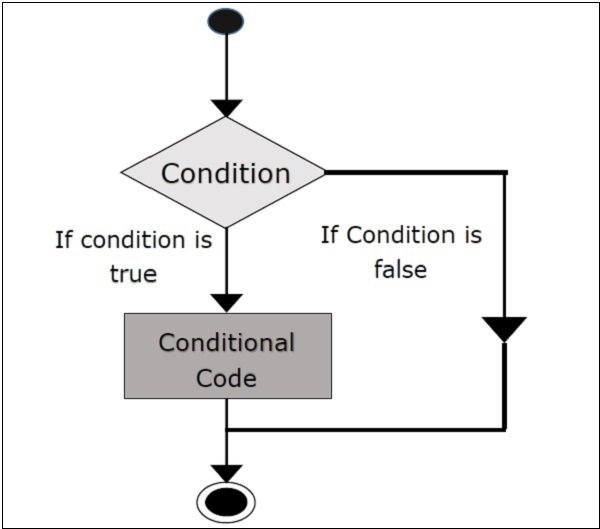
\includegraphics[width=0.7\linewidth]{img/if}
	\caption{Mô tả cách thức hoạt động của câu lệnh if}
\end{figure}
\newpage
\textbf{Ví dụ:} Chương trình nhập vào một số nguyên, nếu số đó là số chẵn thì in ra màn hình:\\
\rule{\linewidth}{0.2mm}\par
\begin{linenumbers}
	\texttt{number = \textcolor{red}{int}(\textcolor{blue}{input}("Type a number: "))}\par
	\texttt{\textcolor{red}{if} number \% 2 == 0:}\par
	\qquad \texttt{\textcolor{blue}{print}("\%d is an even number." \% number)}
\end{linenumbers}
\rule{\linewidth}{0.2mm}\par
\noindent
\resetlinenumber
Kết quả cho ra ở Console:\\
\rule{\linewidth}{0.2mm}\par
\begin{linenumbers}
	\texttt{Type a number: 12}\par
	\texttt{12 is an even number.}
\end{linenumbers}
\rule{\linewidth}{0.2mm}\par
\resetlinenumber
\newpage
\textbf{Ví dụ:}  Kiểm tra tuổi của sinh viên, nếu trên 17 là được chấp nhận:\\
\rule{\linewidth}{0.2mm}\par
\begin{linenumbers}
	\texttt{age = \textcolor{red}{int}(\textcolor{blue}{input}("Type your age: "))}\par
	\texttt{\textcolor{red}{if} age > 17: }\par
	\qquad \texttt{\textcolor{blue}{print}("Accepted!")}
\end{linenumbers}
\rule{\linewidth}{0.2mm}\par
\noindent
\resetlinenumber
Kết quả cho ra ở Console:\\
\rule{\linewidth}{0.2mm}\par
\begin{linenumbers}
	\texttt{Type your age: 16}\par
\end{linenumbers}
\rule{\linewidth}{0.2mm}\par
\resetlinenumber
\newpage
\subsection{Câu lệnh if - else}
Ở câu lệnh if, chương trình chỉ thực thi khối lệnh nếu điều kiện vào là đúng. Trong nhiều trường hợp, ta cũng cần phải xử lý chương trình khi điều kiện vào là sai. Việc sử dụng từ khoá \texttt{else} sẽ giải quyết được trường hợp trên.\par
Cấu trúc của câu lệnh if - else:\par
\texttt{if <condition>:}\par
\qquad \texttt{//if block's code}\par
\texttt{else:}\par
\qquad \texttt{//else block's code}\par
\begin{figure}[h]
	\centering
	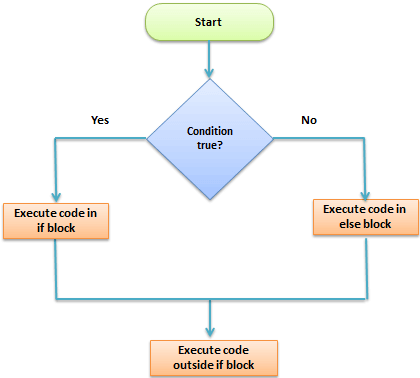
\includegraphics{img/if_else}
	\caption{Mô tả cách thức hoạt động của câu lệnh if - else}
\end{figure}
\newpage
\textbf{Ví dụ:} Chương trình nhập vào một số nguyên, kiểm tra đó là số chẵn hay lẻ:\\
\rule{\linewidth}{0.2mm}\par
\begin{linenumbers}
	\texttt{number = \textcolor{red}{int}(\textcolor{blue}{input}("Type a number: "))}\par
	\texttt{\textcolor{red}{if} number \% 2 == 0:}\par
	\qquad \texttt{\textcolor{blue}{print}("\%d is an even number." \% number)}\par
	\texttt{\textcolor{red}{else}:}\par
	\qquad \texttt{\textcolor{blue}{print}("\%d is an odd number." \% number)}\par
\end{linenumbers}
\rule{\linewidth}{0.2mm}\par
\noindent
\resetlinenumber
Kết quả cho ra ở Console:\\
\rule{\linewidth}{0.2mm}\par
\begin{linenumbers}
	\texttt{Type a number: 11}\par
	\texttt{11 is an odd number.}
\end{linenumbers}
\rule{\linewidth}{0.2mm}\par
\resetlinenumber
\newpage
\textbf{Ví dụ:} Chương trình xếp loại, với điểm >= 8 xếp loại giỏi, >= 7 xếp loại khá và còn lại là trung bình:\\
\rule{\linewidth}{0.2mm}\par
\begin{linenumbers}
	\texttt{score = \textcolor{red}{float}(\textcolor{blue}{input}("Type your score: "))}\par
	\texttt{\textcolor{red}{if} score >= 8:}\par
	\qquad \texttt{\textcolor{blue}{print}("Excellent")}\par
	\texttt{\textcolor{red}{else}:}\par
	\qquad \texttt{\textcolor{red}{if} score >= 7:}\par
	\qquad \qquad \texttt{\textcolor{blue}{print}("Good")}\par
	\qquad \texttt{\textcolor{red}{else}:}\par
	\qquad \qquad \texttt{\textcolor{blue}{print}("Medium")}\par
\end{linenumbers}
\rule{\linewidth}{0.2mm}\par
\noindent
\resetlinenumber
Kết quả cho ra ở Console:\\
\rule{\linewidth}{0.2mm}\par
\begin{linenumbers}
	\texttt{Type your score: 6.2}\par
	\texttt{Medium}
\end{linenumbers}
\rule{\linewidth}{0.2mm}\par
\resetlinenumber
\newpage
\subsection{Câu lệnh if - elif (else if) - else}
Trong trường hợp cần xét nhiều hơn 2 điều kiện, thay vì sử dụng \texttt{else: if <condition>:}, ta có thể viết gọn thành \texttt{elif}.\par
Cấu trúc của câu lệnh if - elif - else:\par
\texttt{if <condition>:}\par
\qquad \texttt{//if block's code}\par
\texttt{elif <condition>:}\par
\qquad \texttt{//elif block's code}\par
\texttt{[elif <condition>:}\par
\qquad \texttt{//elif block's code]}\par
\texttt{[...]}\par
\texttt{else:}\par
\qquad \texttt{//else block's code}\par
\begin{figure}[h]
	\centering
	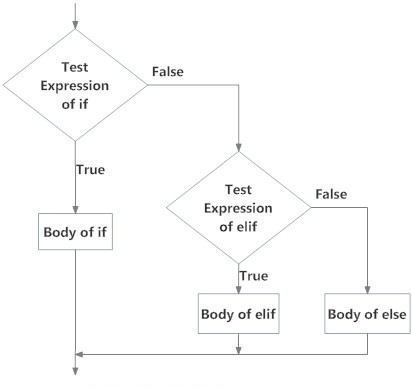
\includegraphics{img/if_elif}
	\caption{Mô tả cách thức hoạt động của câu lệnh if - elif - else}
\end{figure}
\newpage
\textbf{Ví dụ:} Chương trình nhập vào một số, kiểm tra số đó là số âm, số dương hay số 0:\\
\rule{\linewidth}{0.2mm}\par
\begin{linenumbers}
	\texttt{number = \textcolor{red}{float}(\textcolor{blue}{input}("Type a number: "))}\par
	\texttt{\textcolor{red}{if} number > 0:}\par
	\qquad \texttt{\textcolor{blue}{print}("\%.3f is a positive number." \% number)}\par
	\texttt{\textcolor{red}{elif} number < 0:}\par
	\qquad \texttt{\textcolor{blue}{print}("\%.3f is a negative number." \% number)}\par
	\texttt{\textcolor{red}{else}:}\par
	\qquad \texttt{\textcolor{blue}{print}("The number is 0.")}\par
\end{linenumbers}
\rule{\linewidth}{0.2mm}\par
\noindent
\resetlinenumber
Kết quả cho ra ở Console:\\
\rule{\linewidth}{0.2mm}\par
\begin{linenumbers}
	\texttt{Type a number: -18.25}\par
	\texttt{-18.250 is a negative number.}
\end{linenumbers}
\rule{\linewidth}{0.2mm}\par
\resetlinenumber
\newpage
\textbf{Ví dụ:} Chương trình giải phương trình bậc 2:\\
\rule{\linewidth}{0.2mm}\par
\begin{linenumbers}
	\texttt{\textcolor{red}{import} math}\par
	\bigskip
	\texttt{a = \textcolor{red}{int}(\textcolor{blue}{input}("Type your first coefficient: "))}\par
	\texttt{b = \textcolor{red}{int}(\textcolor{blue}{input}("Type your second coefficient: "))}\par
	\texttt{c = \textcolor{red}{int}(\textcolor{blue}{input}("Type your third coefficient: "))}\par
	\texttt{delta = b * b - 4 * a * c}\par
	\texttt{\textcolor{red}{if} delta < 0:}\par
	\qquad \texttt{\textcolor{blue}{print}("The equation has no solution.")}\par
	\texttt{\textcolor{red}{elif} delta == 0:}\par
	\qquad \texttt{x = - b / (2 * a)}\par
	\qquad \texttt{\textcolor{blue}{print}("x = \%.2f" \% x)}\par
	\texttt{\textcolor{red}{else}:}\par
	\qquad \texttt{x1 = (-b - math.sqrt(delta)) / (2 * a)}\par
	\qquad \texttt{x2 = (-b + math.sqrt(delta)) / (2 * a)}\par
	\qquad \texttt{\textcolor{blue}{print}("x1 = \%.2f, x2 = \%.2f" \% (x1, x2))}\par
\end{linenumbers}
\rule{\linewidth}{0.2mm}\par
\noindent
\resetlinenumber
Kết quả cho ra ở Console với ví dụ giải phương trình $2x^2 + 3x - 1$:\\
\rule{\linewidth}{0.2mm}\par
\begin{linenumbers}
	\texttt{Type your first coefficient: 2}\par
	\texttt{Type your second coefficient: 3}\par
	\texttt{Type your third coefficient: 1}\par
	\texttt{x1 = -1.00, x2 = -0.50}
\end{linenumbers}
\rule{\linewidth}{0.2mm}\par
\resetlinenumber
\newpage
\textbf{Ví dụ:} Chương trình giải hệ phương trình bậc nhất hai ẩn:\\
\rule{\linewidth}{0.2mm}\par
\begin{linenumbers}
	\texttt{a1 = \textcolor{red}{int}(\textcolor{blue}{input}("a1 = "))}\par
	\texttt{b1 = \textcolor{red}{int}(\textcolor{blue}{input}("b1 = "))}\par
	\texttt{c1 = \textcolor{red}{int}(\textcolor{blue}{input}("c1 = "))}\par
	\medskip
	\texttt{a2 = \textcolor{red}{int}(\textcolor{blue}{input}("a2 = "))}\par
	\texttt{b2 = \textcolor{red}{int}(\textcolor{blue}{input}("b2 = "))}\par
	\texttt{c2 = \textcolor{red}{int}(\textcolor{blue}{input}("c2 = "))}\par
	\medskip
	\texttt{d = a1 * b2 - a2 * b1}\par
	\texttt{dx = c1 * b2 - c2 * b1}\par
	\texttt{dy = a1 * c2 - a2 * c1}\par
	\medskip
	\texttt{\textcolor{red}{if} d == 0 and dx == dy and dx == 0:}\par
	\qquad \texttt{\textcolor{blue}{print}("This equations has an infinite number of solutions.")}\par
	\texttt{\textcolor{red}{elif} d == 0 and dx != dy:}\par
	\qquad \texttt{\textcolor{blue}{print}("This equations has no solution.")}\par
	\texttt{\textcolor{red}{else}:}\par
	\qquad \texttt{x = dx / d}\par
	\qquad \texttt{y = dy / d}\par
	\qquad \texttt{\textcolor{blue}{print}("x = \%.2f, y = \%.2f" \% (x, y))}\par
\end{linenumbers}
\rule{\linewidth}{0.2mm}\par
\noindent
\resetlinenumber
Kết quả cho ra ở Console với ví dụ giải hệ phương trình
$\begin{cases}
	x - y = 1\\
	x + y = 3
\end{cases}$:\par
\noindent
\rule{\linewidth}{0.2mm}\par
\begin{linenumbers}
	\texttt{a1 = 1}\par
	\texttt{b1 = -1}\par
	\texttt{c1 = 1}\par
	\texttt{a2 = 1}\par
	\texttt{b2 = 1}\par
	\texttt{c2 = 3}\par
	\texttt{x = 2.00, y = 1.00}
\end{linenumbers}
\rule{\linewidth}{0.2mm}\par
\resetlinenumber
\newpage
\subsection{Switch - case}
Python không có cấu trúc switch case đơn giản. Thay vào đó, chúng ta có thể sử dụng một dictionary để ánh xạ đến các case.\par
Cấu trúc một dictionary:\par
\texttt{<name of dictionary> = \{}\par
\qquad \texttt{<key 1>: <value 1>,}\par
\qquad \texttt{[<key 2>: <value 2>,]}\par
\qquad \texttt{[<key 3>: <value 3>,]}\par
\qquad \texttt{[...]}\par
\texttt{\}}\par
Ta sử dụng hàm \texttt{get(<key>, <value if key not found>)} để lấy value từ một key đã biết trước.
\newpage
\textbf{Ví dụ:} Chương trình nhập vào tháng dạng số nguyên, xuất ra tên tháng:\\
\rule{\linewidth}{0.2mm}\par
\begin{linenumbers}
	\texttt{\textcolor{red}{def} get\_month\_by\_number(month):}\par
	\qquad \texttt{switch = \{}\par
	\qquad \qquad \texttt{1: 'January',}\par
	\qquad \qquad \texttt{2: 'February',}\par
	\qquad \qquad \texttt{3: 'March',}\par
	\qquad \qquad \texttt{4: 'April',}\par
	\qquad \qquad \texttt{5: 'May',}\par
	\qquad \qquad \texttt{6: 'June',}\par
	\qquad \qquad \texttt{7: 'July',}\par
	\qquad \qquad \texttt{8: 'August',}\par
	\qquad \qquad \texttt{9: 'September',}\par
	\qquad \qquad \texttt{10: 'October',}\par
	\qquad \qquad \texttt{11: 'November',}\par
	\qquad \qquad \texttt{12: 'December'}\par
	\qquad \texttt{\}}\par
	\qquad \texttt{\textcolor{red}{return}  switch.get(month, 'Month must be less than 13 and greater than 0.')}\par
	\bigskip
	\texttt{month = \textcolor{red}{int}(\textcolor{blue}{input}("Type your month: "))}\par
	\texttt{\textcolor{blue}{print}(get\_month\_by\_number(month))}\par
\end{linenumbers}
\rule{\linewidth}{0.2mm}\par
\noindent
\resetlinenumber
Kết quả cho ra ở Console:\\
\rule{\linewidth}{0.2mm}\par
\begin{linenumbers}
	\texttt{Type your month: 8}\par
	\texttt{August}\par
\end{linenumbers}
\rule{\linewidth}{0.2mm}\par
\resetlinenumber
\newpage
\textbf{Ví dụ:} Chương trình nhập vào tháng dạng số nguyên, xuất số ngày trong tháng:\\
\rule{\linewidth}{0.2mm}\par
\begin{linenumbers}
	\texttt{\textcolor{red}{def} get\_month\_by\_number(month):}\par
	\qquad \texttt{switch = \{}\par
	\qquad \qquad \texttt{1: 'January', 2: 'February', 3: 'March', 4: 'April', }\par
	\qquad \qquad \texttt{5: 'May', 6: 'June', 7: 'July', 8: 'August', }\par
	\qquad \qquad \texttt{9: 'September', 10: 'October', 11: 'November', 12: 'December'}\par
	\qquad \texttt{\}}\par
	\medskip
	\texttt{\textcolor{red}{def} get\_day\_of\_february():}\par
	\qquad \texttt{year = \textcolor{red}{int}(\textcolor{blue}{input}("Type a year: "))}\par
	\qquad \texttt{\textcolor{red}{if} year \% 400 == 0 or (year \% 4 == 0 and year \% 100 != 0):}\par
	\qquad \qquad \texttt{return 29}\par
	\qquad \texttt{return 28}\par
	\medskip
	\texttt{\textcolor{red}{def} get\_day\_of\_month(month):}\par
	\qquad \texttt{switch = \{}\par
	\qquad \qquad \texttt{1: 31, 2: get\_day\_of\_february(),}\par
	\qquad \qquad \texttt{3: 31, 4: 30,}\par
	\qquad \qquad \texttt{5: 31, 6: 30,}\par
	\qquad \qquad \texttt{7: 31, 8: 31,}\par
	\qquad \qquad \texttt{9: 30, 10: 31,}\par
	\qquad \qquad \texttt{11: 30, 12: 31}\par
	\qquad \texttt{\}}\par
	\qquad \texttt{\textcolor{red}{return}  switch.get(month, 'Month must be less than 13 and greater than 0.')}\par
	\medskip
	\texttt{month = \textcolor{red}{int}(\textcolor{blue}{input}("Type a month: "))}\par
	\texttt{\textcolor{blue}{print}(get\_month\_by\_number(month), 'has', get\_day\_of\_month(month), 'days.')}\par
\end{linenumbers}
\rule{\linewidth}{0.2mm}\par
\noindent
\resetlinenumber
Kết quả cho ra ở Console:\\
\rule{\linewidth}{0.2mm}\par
\begin{linenumbers}
	\texttt{Type a month: 2}\par
	\texttt{Type a year: 2003}\par
	\texttt{February has 28 days.}\par
\end{linenumbers}
\rule{\linewidth}{0.2mm}\par
\resetlinenumber
\newpage




\newpage